\section{Branching Dueling Q-Network (BDQ)}

\begin{figure}[htbp] 
    \begin{subfigure}{0.31\textwidth}
      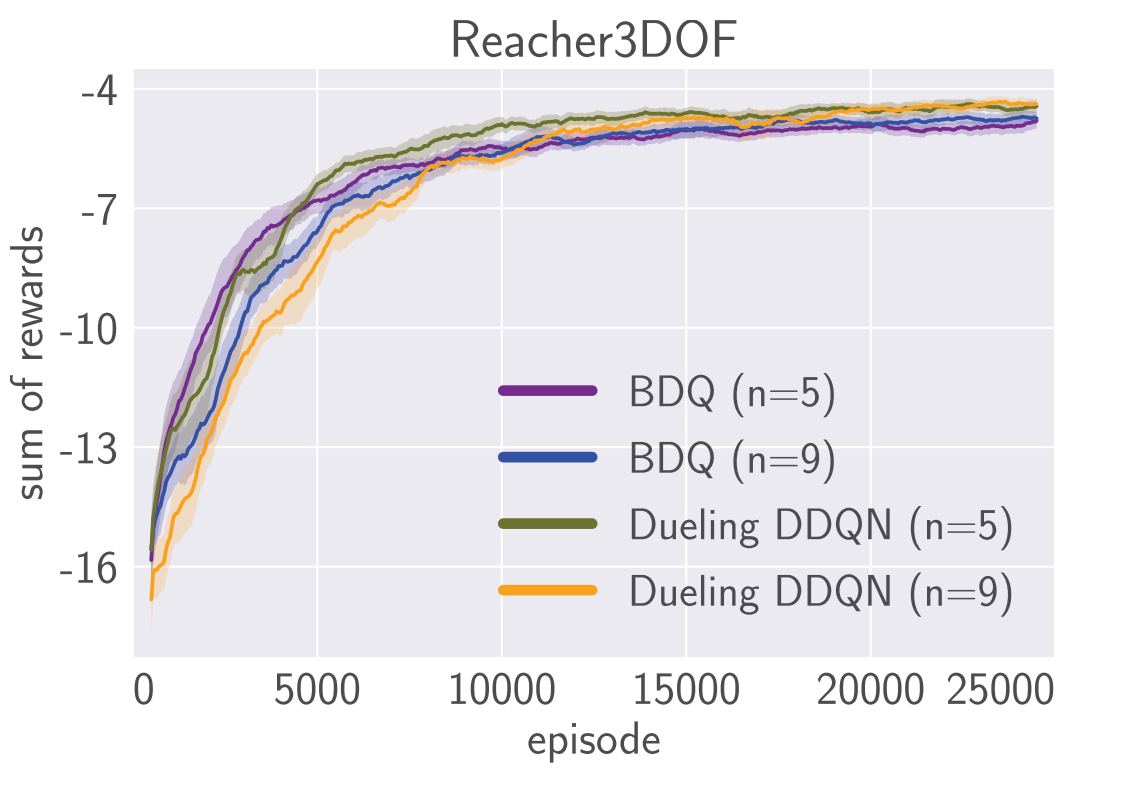
\includegraphics[width=\linewidth]{figures/BDQ1.png}
      \caption{} \label{fig:1a}
    \end{subfigure}%
    \hspace*{\fill}   % maximize separation between the subfigures
    \begin{subfigure}{0.31\textwidth}
      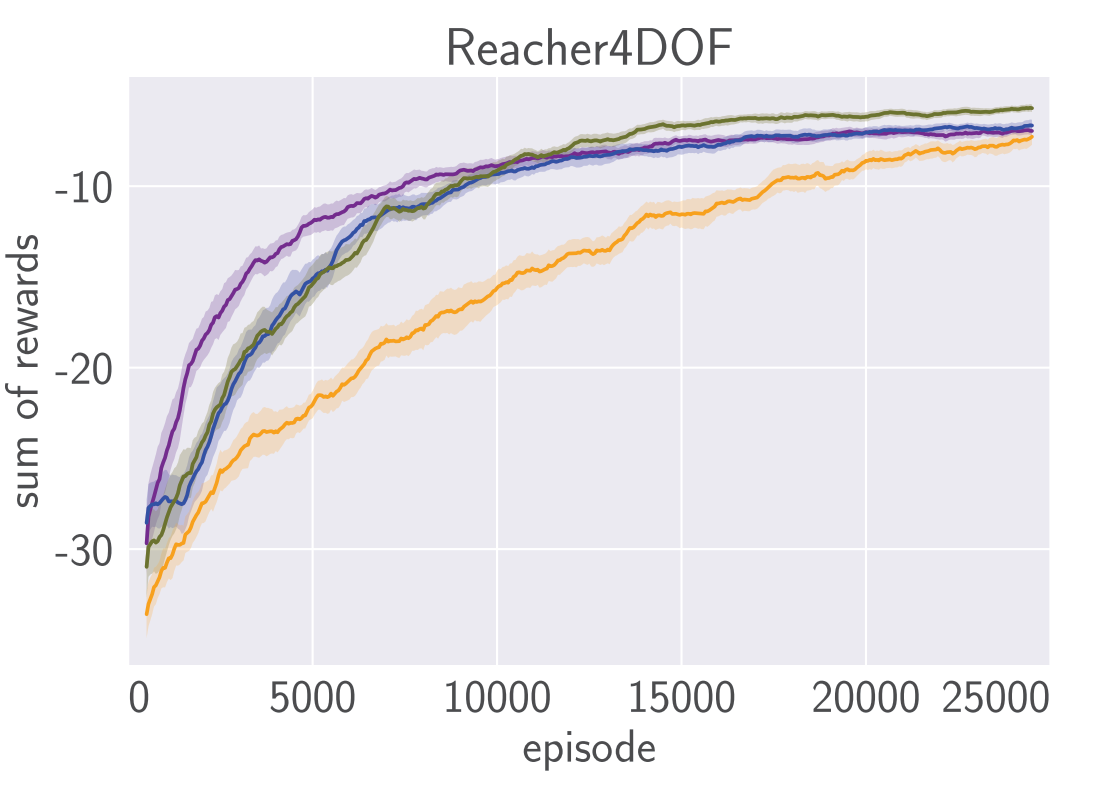
\includegraphics[width=\linewidth]{figures/BDQ2.png}
      \caption{} \label{fig:1b}
    \end{subfigure}%
    \hspace*{\fill}   % maximize separation between the subfigures
    \begin{subfigure}{0.31\textwidth}
      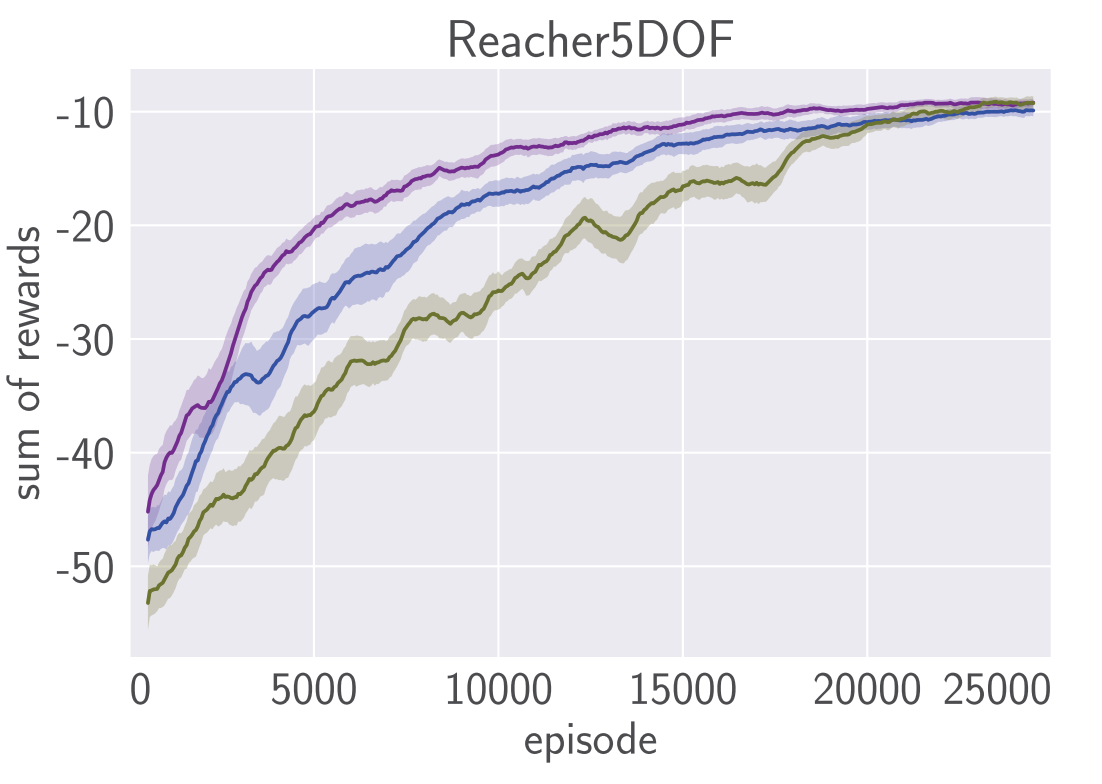
\includegraphics[width=\linewidth]{figures/BDQ3.png}
      \caption{} \label{fig:1b}
    \end{subfigure}%

\caption{BDQ performances compared to Dueling-Double-DQN with increasing action spaces \label{fig:BDQvsDDQN}}
\end{figure}

BDQ is our test algorithm. Tavakoli et al. developed BDQ as a variant of Dueling Double DQN \cite{Tavakoli2018}. They aimed to solve the intractability of the DQN algorithm on high dimensional continuous tasks. The key feature of their algorithm is the shared module. The shared module representation allowed the DQN algorithm to cope with the intractability problem. Tavakoli et al. showed that their network could output multi-dimensional actions without convergence issues. They believe the stability of the structure is due to the encoded latent representation of the input in the shared module.

Their results stress that, especially in higher dimensional action spaces, BDQ performs better than Double-dueling DQN implementation \ref{fig:BDQvsDDQN}. Even compared to proven algorithms, like DDPG, it cannot reach the level of BDQ. Although researchers at google deep mind presented in 2016 that the DDPG algorithm outperforms DQN variants at almost every task \cite{Lillicrap2016}, Tavakoli et al. proved the opposite that BDQ shows better performance than DDPG on Humanoid walking benchmark task \ref{fig:bdqvsddpg}.

\begin{figure}[htbp] 
    \centering
    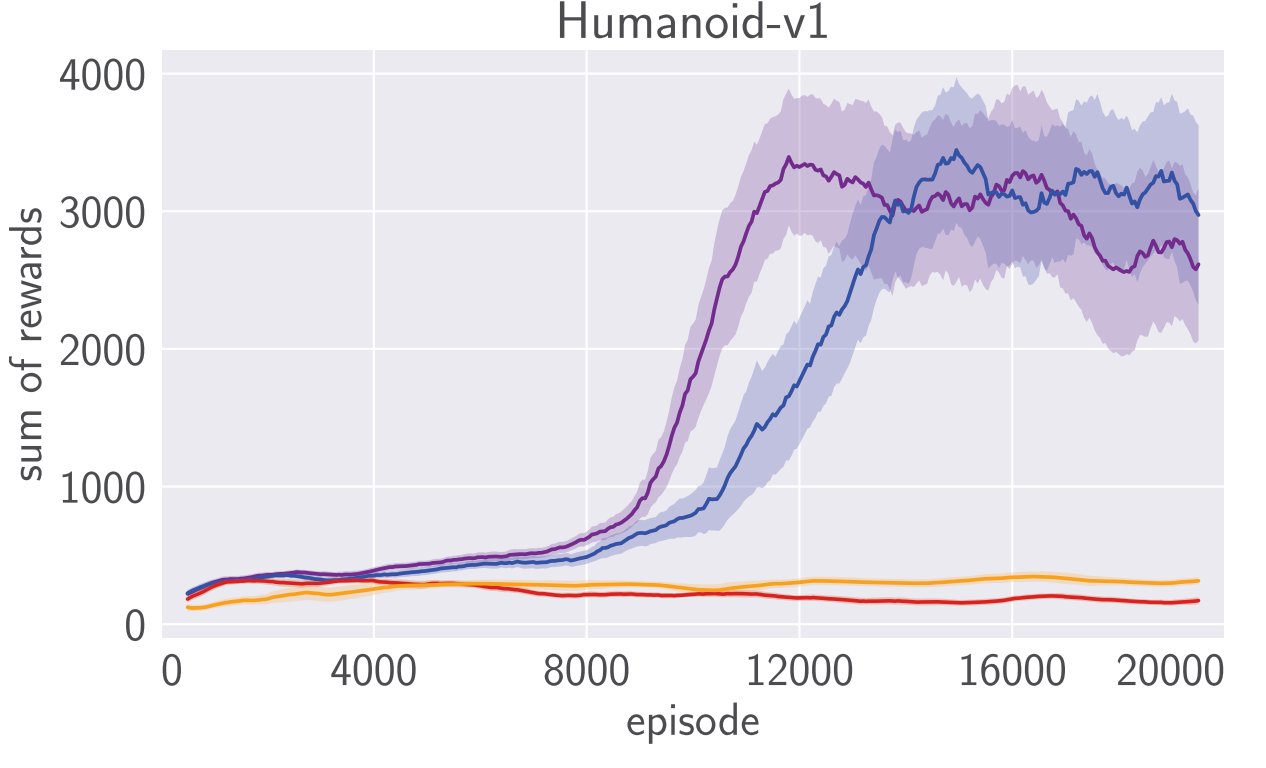
\includegraphics[width=0.7\textwidth]{figures/BDQvsDDPG}
    \caption{Blue line represents }
    \label{fig:bdqvsddpg}
\end{figure}

In this section, we will go through the implementation details of BDQ. The authors of the BDQ article provided their implementation of BDQ on Github. Based on the original code and the insights from the article, we implemented our version of BDQ on stable-baselines codebase. As a result, we avoid the save, load model issues from BDQ original code, and use new features available such as callback structure, parameter manipulation, warn starting, etc. 


\subsection{BDQ Implementation}


\begin{figure}[htbp] 
    \centering
    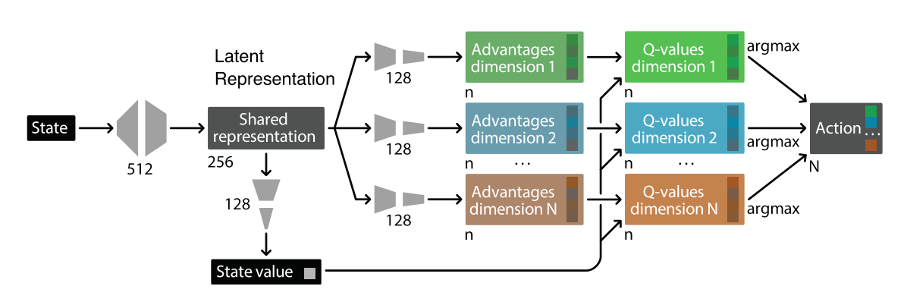
\includegraphics[width=1.0\textwidth]{figures/bdq_network.png}
    \caption{BDQ network representation}
    \label{fig:bdq_net}
\end{figure}

BDQ adopts new improvements from the DQN algorithm, such as double-q function, dueling architecture, prioritized replay. One crucial design decision is they choose to keep the same state-value estimation for each action branch, while advantage functions are unique to every stream of actions \ref{fig:bdq_net}. Later they combine common state-value estimate and advantage function in the aggregation layer. This approach helps with the generalization of the actions in similar states by reducing the overfitting of action branches. Therefore, they can scale up to more complex and higher dimensional tasks, where Dueling-Double DQN becomes intractable.

Another key difference of BDQ is the aggregation layer; they subtract the mean advantage value from the advantage value of an individual branch. Then, sum up the result to calculate the Q-function value of each branch \ref{eq:bdq_betterx}. Although the lack of identifiability problem, they achieve better results than the theoretically proven max reduction method \ref{eq:bdq_proven}.

\begin{equation}
    Q_d(s, a_d) = V(s) + \Big(A_d(s, a_d) - \frac{1}{n} \sum\limits_{a_d'\in A_d}A_d(s, a_d')\Big)
    \label{eq:bdq_better}
\end{equation}


\begin{equation}
    Q_d(s, a_d) = V(s) + \Big(A_d(s, a_d) - \max\limits_{a_d'\in A_d}A_d(s, a_d')\Big)
    \label{eq:bdq_proven}
\end{equation}


TD-target definition of BDQ also differs from DDQN. Where DDQN based approach calculates the individual TD-target for every branch \ref{eq:ddqn_tdtarget}, BDQ sets one global target for all actions by taking the mean of the max Q-function variable in the TD-target equation \ref{eq:bdq_tdtarget}. In our opinion, a common TD-target for all branches of BDQ underlines the dependency between action branches and forces them to act in collaboration.

\begin{equation}
    y_d = r + \gamma Q{_d^-}\Big(s', \arg\max\limits_{a_d'\in A_d}Q_d(s', a'_d)\Big)
    \label{eq:ddqn_tdtarget}
\end{equation}

\begin{equation}
    y = r + \gamma \frac{1}{N} \sum\limits_d Q{_d^-}\Big(s', \arg\max\limits_{a_d'\in A_d}Q_d(s', a'_d)\Big)
    \label{eq:bdq_tdtarget}
\end{equation}


Analogous to the TD-target definition, they express loss differently than the DDQN counterpart. BDQ authors calculate the loss first by taking the mean of the squared TD-error over the branches and then taking the expectation of this score \ref{eq:bdq_loss}. Identical to the TD-target calculation, loss definition also helps the action branches to act dependent on each other.

\begin{equation}
    L = \mathop{\mathbb{E}}_{(s,a,r,s')\sim D} \Big[\frac{1}{N}\sum\limits_d(y_d-Q_d(s,a_d))^2]
    \label{eq:bdq_loss}
\end{equation}

Exploration-exploitation trade-off is still on-going research in RL. Nevertheless, researchers assume better-exploring algorithms have the edge over weakly exploring algorithms, such as SAC with a robust entropy-based exploration approach is considered the best exploring algorithm and the state-of-art RL algorithm \cite{Haarnoja2018}. BDQ original code offers two different exploration approach, epsilon greedy and gaussian noise. Since epsilon-greedy usually used with discrete DQN based algorithms, the authors found it inadequate to explore continuous spaces. Instead of epsilon-greedy, they recommended the use of Gaussian-noise for better performance.

BDQ follows the same pseudocode of double-DQN(\ref{fig:bdqalgo}) with dueling and branching network extensions, which does not affect the underlying algorithm.

\begin{figure}[htbp] 
    \centering
    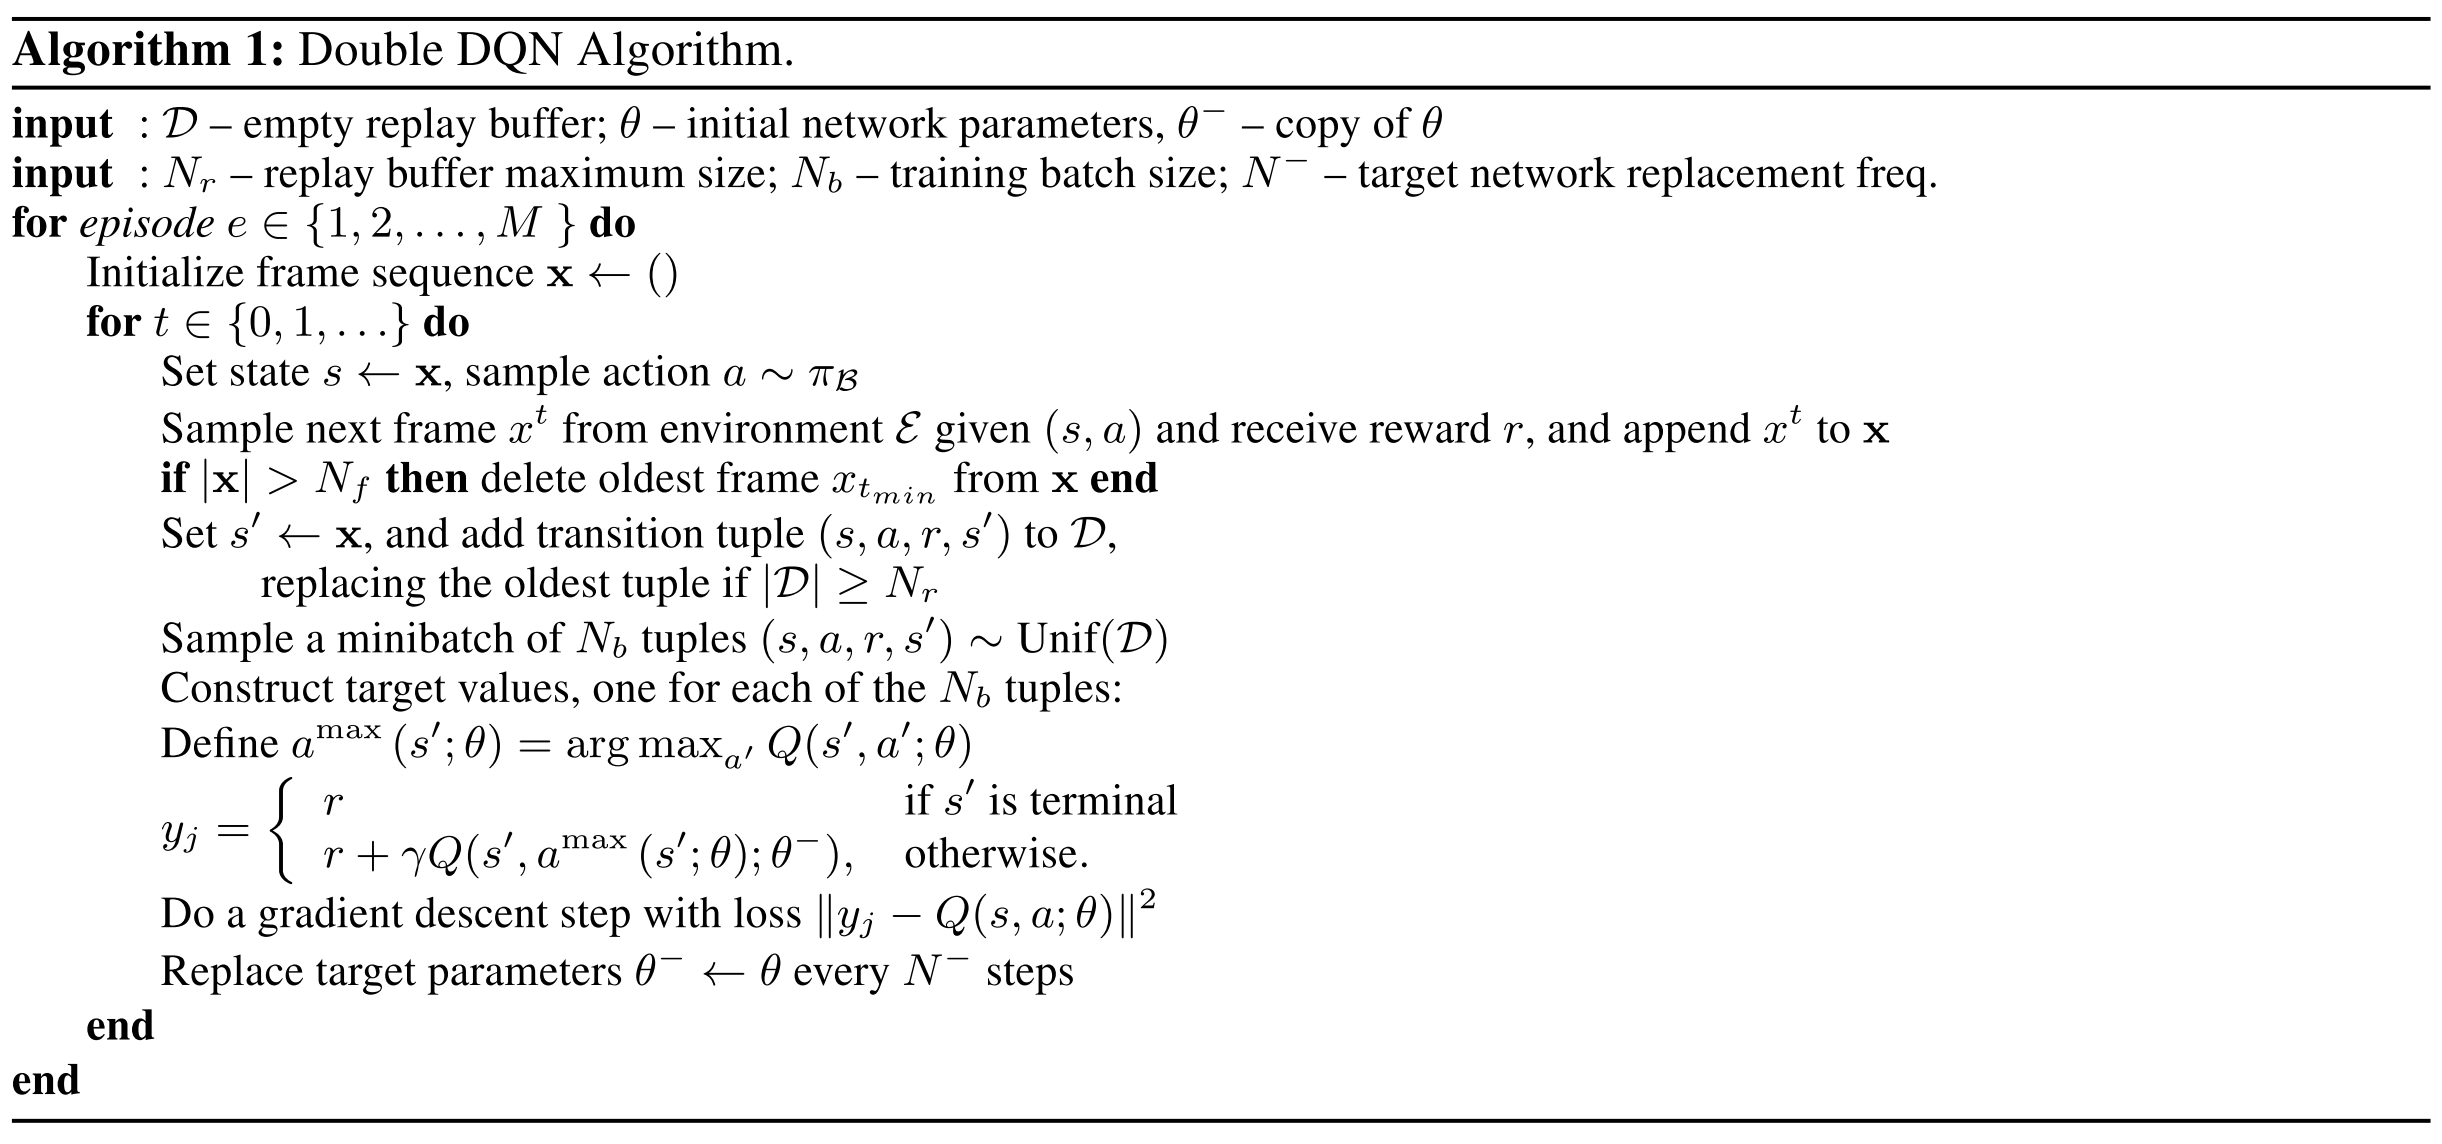
\includegraphics[width=1.0\textwidth]{figures/BDQalgo}
    \caption{Double-DQN pseudocode \cite{Wang2016}}
    \label{fig:bdqalgo}
\end{figure}
